%%%% ijcai23.tex

\typeout{IJCAI--23 Instructions for Authors}

% These are the instructions for authors for IJCAI-23.

\documentclass{article}
\pdfpagewidth=8.5in
\pdfpageheight=11in

% The file ijcai23.sty is a copy from ijcai22.sty
% The file ijcai22.sty is NOT the same as previous years'
\usepackage{ijcai23}

% Use the postscript times font!
\usepackage{times}
\usepackage{soul}
\usepackage{url}
\usepackage[hidelinks]{hyperref}
\usepackage[utf8]{inputenc}
\usepackage[small]{caption}
\usepackage{graphicx}
\usepackage{amsmath}
\usepackage{amsthm}
\usepackage{booktabs}
\usepackage{algorithm}
\usepackage{amsfonts}
% \usepackage{algorithmic}
\usepackage{algpseudocode}
\usepackage[switch]{lineno}
\usepackage{multirow}
\usepackage{subfigure}

% Comment out this line in the camera-ready submission
\linenumbers

\urlstyle{same}

% the following package is optional:
%\usepackage{latexsym}

% See https://www.overleaf.com/learn/latex/theorems_and_proofs
% for a nice explanation of how to define new theorems, but keep
% in mind that the amsthm package is already included in this
% template and that you must *not* alter the styling.
\newtheorem{example}{Example}
\newtheorem{theorem}{Theorem}

% Following comment is from ijcai97-submit.tex:
% The preparation of these files was supported by Schlumberger Palo Alto
% Research, AT\&T Bell Laboratories, and Morgan Kaufmann Publishers.
% Shirley Jowell, of Morgan Kaufmann Publishers, and Peter F.
% Patel-Schneider, of AT\&T Bell Laboratories collaborated on their
% preparation.

% These instructions can be modified and used in other conferences as long
% as credit to the authors and supporting agencies is retained, this notice
% is not changed, and further modification or reuse is not restricted.
% Neither Shirley Jowell nor Peter F. Patel-Schneider can be listed as
% contacts for providing assistance without their prior permission.

% To use for other conferences, change references to files and the
% conference appropriate and use other authors, contacts, publishers, and
% organizations.
% Also change the deadline and address for returning papers and the length and
% page charge instructions.
% Put where the files are available in the appropriate places.


% PDF Info Is REQUIRED.
% Please **do not** include Title and Author information
\pdfinfo{
/TemplateVersion (IJCAI.2023.0)
}

\title{A Relation-specific Entropy-based Ensemble Approach for Knowledge Graph}


% Single author syntax
% \author{
%     Hwawoo Jeon^{1,2}, Yoonseob Lim^{1} and Yong Suk Choi^{2}
%     \affiliations
%     Affiliation
%     \emails
%     email@example.com
% }

% Multiple author syntax (remove the single-author syntax above and the \iffalse ... \fi here)
% \iffalse
\author{
Hwawoo Jeon$^{1,2}$\and
Yoonseob Lim$^{1,3}$\And
Yong Suk Choi$^2$
\affiliations
$^1$Center for Intelligent \& Interactive Robotics\unskip,
Korea Institute of Science and Technology\unskip, 136-791\unskip, Seoul\unskip, Korea\\
$^2$The Division of Computer Science and Engineering\unskip,
Hanyang University\unskip, 04763\unskip, Seoul\unskip, Korea\\
$^3$Department of HY-KIST Bio-convergence\unskip,
Hanyang University\unskip, 04763\unskip, Seoul\unskip, Korea\\
\emails
\{feelgood88, yslim\}@kist.re.kr,
cys@hanyang.ac.kr
}
% \fi

\begin{document}

\maketitle

\begin{abstract}
    Knowledge Graph Embedding(KGE) aims to represent entities and relationships from knowledge graphs(KGs) in vector spaces. Existing KGE methods often focus narrowly on specific patterns, which constrains their inferential capabilities to predict diverse relationship patterns. In response to this limitation, we introduce a relation-specific entropy-based KG ensemble approach, denoted as ERSE. We assume that the entropy of similarity distribution of feature vectors is a reliable indicator of the inference potential for particular relations. On the basis of this hypothesis, ERSE utilizes relation-specific ensemble weights, determined by the entropy of feature vector similarity derived from the base model and independent training data. Moreover, ERSE is designed to be flexible in that it adopts combining base models using normalized entropy measurements in order to effectively be applied to various KG datasets and complex prediction environments. Our experiments on the FB15K and FB15k237 datasets, using four translation-based KGE methods (TransE, TransH, TransR, and TransD) as base models, show that ERSE surpasses both of each single-model and conventional ensemble approaches in terms of prediction accuracy. These results corroborate our hypothesis that the relation-specific entropy of feature vector similarity can take good effect on inference performance of KGE. The code is public at ~\hyperlink{https://github.com/HW-Jeon/ERSE}{https://github.com/HW-Jeon/ERSE}.

\end{abstract}

\section{Introduction}

In artificial intelligence, Knowledge Graphs (KGs) play a pivotal role by structuring and representing extensive knowledge. They represent real-world objects and abstract concepts through entities, relationships, and semantic descriptions. Prominent KGs like FreeBase, WordNet, and DBpedia have been instrumental in various applications, including question-answering and recommendation systems~\cite{10.1093/bib/bbac481,zheng2021knowledge,chen2021topic}.

However, KGs often face the challenge of incompleteness due to the intricate nature of representing the myriad relationships between entities. To address this, knowledge graph embeddings (KGEs) have been proposed. KGEs, employing link-prediction techniques, aim to infer missing links, thereby mitigating KG incompleteness. In this process, KGEs transform KG elements, denoted as triple facts $(h, r, t)$, into a continuous vector space, preserving the KG's structure. The likelihood of a triple is then assessed using a scoring function. Recent advancements have seen the emergence of diverse KGE models~\cite{ji2021survey}, utilizing varied representation spaces and scoring functions: semantic matching models featuring tensor factorization like RESCAL, translational distance models following TransE's translational-principle, complex vector models utilizing complex space as introduced in ComplEx, and models based on neural networks. Despite these developments, no single KGE model has successfully modeling all KG attributes, such as relation patterns (symmetric, anti-symmetric, inverse, composition, hierarchy) and inter-entity (1-to-1, 1-to-N, N-to-1, N-to-N) relationships~\cite{WANG20221041,choi2020approach}. This limitation underscores the need for models that integrate KG information more comprehensively.

Ensemble learning approaches, which generally known to outperform single learners, have seen significant success in machine learning. This concept has been effectively adapted to the context of KGEs, starting with the work of Krompaß and Tresp~\cite{krompass2015ensemble}. Various approaches have been proposed, including committee-based models that derive a final score from a KGEs committee~\cite{choi2020approach}, ensembles of identical KGE models embedded in lower dimensions~\cite{9533372}, and recent methods employing probabilistic ensemble weights~\cite{WANG20221041}.

This paper introduces a novel approach, the ERSE (knowledge graph Ensemble with Relation-Specific Entropy), which focuses on utilizing the entropy of similarity distribution of prediction vector, denoted as feature vector, in each model's representation vector space rather than individual prediction scores of base-model. This methodology stems from the principles of Causal Entropy Force and the proven effectiveness of entropy in complex systems performance evaluation, like the cross-entropy method~\cite{wissner2013causal, de2005tutorial}. In briefly, ERSE extracts triples with specific relations, filtering prediction vectors, based on each model's prediction ranking, and then calculates relation-specific ensemble weights based on the entropy of these feature vector. This method, applied to the FB15K and FB15k237 datasets using four translation-based KGE methods(TransE, TransH, TransR, TransD), demonstrates superior predictive accuracy compared to both single-model and general ensemble approaches.

Our paper's contributions include:
\begin{itemize}
    \item We proposing an ensemble mechanism based on the embedded feature vectors in each base model's representation space;
    \item We propose a ensemble approach with entropy as ensemble weights; 
    \item Demonstrating through experiments that the entropy of similarity distribution of feature vectors is a valid indicator of a model's predictive performance.
\end{itemize}


The remainder of this paper is structured as follows: Section ~\ref{RelatedWork} reviews related works on KGE and ensemble learning. Section ~\ref{Method} details our method. Section ~\ref{Exper} presents experimental results and analyses. Concluding remarks are provided in Section ~\ref{Conclusion}.

\section{Related Work}
\label{RelatedWork}
Before proceeding, we introduce our mathematical notations. A triplet is denoted as $(h, r, t)$, with the corresponding column vectors represented by lowercase letters $h$, $r$, $t$. The sets of entities and relations are indicated by uppercase letters $E$ and $R$, respectively. The set $T$, defined as $\{(h, r, t) : h, t \in E, r \in R\}$, comprises these triplets. This set is further divided into three distinct subsets: $T_{train}$, $T_{val}$, and $T_{test}$, corresponding to training, validation, and testing datasets. The score function is expressed as $s(h, r, t)$. Additional notations are elaborated in relevant sections as needed.


\subsection{Translation-based KGE Models}

\textbf{TransE}~\cite{bordes2013translating}. The TransE model initiated the concept of Translation-Based Embedding models. It conceptualizes each relationship as a form of translation within an embedding space. Here, entities and relations are mapped to a low-dimensional vector space, represented as $h$, $r$, $t$. TransE employs the principle $h + r \approx t$ for translating head entities to tail entities, with the score function defined as: $f(h, r, t) = \Vert h + r - t\Vert_2^2$. Although simple and efficient, TransE primarily effective in modeling 1-to-1 relationships, showing limitations in handling 1-to-N, N-to-1, and N-to-N relations.\\
\textbf{TransH}~\cite{wang2014knowledge}. Addressing limitations of TransE, TransH introduces a relation-specific hyperplane, characterized by a normal vector $\textbf{w}_r$ and a translation vector $d_r$. TransH interprets a relation as a translation operation on a specific hyperplane, determined by a normal vector $\textbf{w}_r$ and a translation vector $d_r$. It projects embeddings $h$ and $t$ onto this hyperplane, resulting in $h_\perp = h - \textbf{w}_r^{\top}h\textbf{w}_r$ and $t_{\perp} = t - \textbf{w}_r^{\top}\textbf{w}_r$, followed by the operation $h_\perp + d_r \approx t_\perp$. The score function for TransH is given by $f(h, r, t) = \Vert h + r - t - \textbf{w}_r(\textbf{w}_r^\top(h - t))\Vert_2^2$.\\
\textbf{TransR}~\cite{lin2015learning}. Both TransE and TransH operate under the premise that entity and relation embeddings coexist in the same space. TransR was proposed from the realization that entities and relations, being fundamentally different, might be better represented in separate vector spaces. TransR differentiates entities and relations by assigning a unique mapping matrix $M_r$ for each relation. The score function in TransR is $f(h, r, t) = \Vert M_r h + r - M_r t\Vert_2^2$, where entity embeddings are transformed by the matrix $M_r$ before applying the translational operation. However, TransR can lead to overfitting in simple relations and underfitting in complex relations, due to the uniform parameter learning across different relation complexities.\\
\textbf{TransD}~\cite{ji2015knowledge}. TransD offer solution to address the overfitting of simple relations and underfitting of complex relations observed in TransR. TransD adopts product of two projection vectors instead of projection matrices. It defines the head and tail projection matrices as $M_rh = r_ph_p^\top + I^{d_r \times d_e}$ and $M_rt = r_pt_p^\top + I^{d_r \times d_e}$, respectively, where $d_r$ and $d_e$ represent the dimensions of relation and entity embeddings. Here, $r_p$ is related to relation $r$, and $h_p$, $t_p$ with the related to head and tail entities. This approach reduces parameter load and improves scalability for extensive KGs.\\
\textbf{TranSparse}~\cite{ji2016knowledge}: The TranSparse model addresses issues of heterogeneity and imbalance in KGs, which previous translation models have overlooked. Heterogeneity in this context means that various relations link a differing number of entity pairs. Meanwhile, imbalance refers to the unequal numbers of head and tail entities within a relation. To tackle these challenges, TranSparse introduces adaptive sparse matrices instead of standard projection matrices. The sparsity of these matrices is tailored according to the quantity of entity pairs or entities associated with each relation. The score function of TranSparse, $f(h,r,t) = \Vert M^h_r (\theta^h_r)h + r - M^t_r (\theta^t_r)t\Vert_{l1/2}^2$, utilizes these adaptive sparse matrices, where $M^h_r (\theta^h_r)$ and $M^t_r (\theta^t_r)$ represent the matrices for head and tail entities, respectively, with $\theta^h_r$ and $\theta^t_r$ indicating their degrees of sparsity.

As reported by Zhang et al.~\cite{zhang-etal-2022-trans}'s study, translation-based KGE models, classified as translational-distance models by Ji et al.\cite{ji2021survey}, are exhibit a same scoring pattern $\Vert \mathsf{R}_h + r - \mathsf{R}_t \Vert$, where $\mathsf{R}_h$ and $\mathsf{R}_t$ are the deformation of $h$ and $t$ . In this paper, we discuss how to combine multiple models by utilizing traditional translation-based models, i.e., TransE, TransH, TransR, and TransD, which share the same scoring pattern, as base-models instead of other models in improve the performance of KGE.  
\subsection{Other Models}
\textbf{ComplEx}~\cite{trouillon2016complex}. ComplEx introduces the concept of embedding KGs in a complex space. This is achieved by employing a complex conjugate. Specifically, ComplEx utilizes the real component of a complex bilinear function to denote the likelihood of a positive relationship. The model's scoring function is defined as $f(h, r, t)=Re(\sum_{i=1}^dh_ir_i\bar{t})$, where $\bar{t}$ denotes the complex conjugate of $t$. This scoring mechanism allows for the representation of triples with asymmetric relationships.\\
\textbf{RotatE}~\cite{sun2019rotate}. Introduced to model relationships in four distinct patterns: symmetry, antisymmetry, inverse, and composition, RotatE conceptualizes each relation as a rotational mapping in complex vector space. This is achieved by embedding the source entity $h$ and the target entity $t$ in a complex vector space, based on Euler's formula: $cos\theta + i sin\theta$. The model's effectiveness is evaluated using the score function $f(h,r,t) = \Vert h \circ r - t \Vert$, quantifying the difference between the inner product of $h$ and $r$, and $t$.

\subsection{Ensemble Learning}
Ensemble methods~\cite{zhou2012ensemble} integrate multiple models into a comprehensive model. These methods generally outperform single models and have been successful in various real-world scenarios~\cite{rivas2022ensembles,osamor2021enhancing}. 

These approaches fall into four main categories: voting, bagging, boosting, and combination strategies. Voting and bagging strategies  are similar in that both sample training data for each learner and then integrate the results, but employ distinct methodologies. In voting strategies, diverse algorithms are trained on identical datasets; their predictions are then amalgamated using averaging or majority voting. This approach, known for reducing overfitting risk, requires careful selection of base models and their integration techniques~\cite{a13010026}. A variant, weighted voting, assigns different weights to each model's predictions, demanding strategy for applying reliable weight based on specific objectives~\cite{osamor2021enhancing}.

Bagging, effective for complex models prone to overfitting, trains each model in parallel, substantially reducing variance. This method, exemplified by Random Forest~\cite{breiman2001random}, however, does not decrease bias in underfitting models and demands higher computational resources. Boosting methods, such as  Adaboost~\cite{freund1996experiments}, iteratively adjust the training data distribution based on previous outputs, enhancing learner performance. Combinatorial strategies independently train learners and merge outcomes through averaging, voting, or additional learners.

Krompaß and Tresp~\cite{krompass2015ensemble} first explored this concept in KGE models, establishing that ensemble predictions outperformed those from individual base models. More recently, Xu et al.~\cite{9533372} demonstrated enhanced performance in KGE models through parallel training at lower dimensions and aggregating scores, compared to training a single higher-dimension model. Additionally, Wang et al.~\cite{WANG20221041} proposed combining different embedding model scores using probabilistic weights, providing a theoretical framework for optimal parameter calculation in ensemble models and predicting link prediction rates.More resently, Wang et al.~\cite{WANG20221041} presented to combine the scores of different embedding models by using a probabilistic weights and theoretical framework to calculate the optimal parameters for the ensemble model and predict its corresponding link prediction rate.

\section{Method}
\label{Method}
\bgroup
\begin{figure*}[t]
  \centering \makeatletter\IfFileExists{Images/Figure1_v2.png}{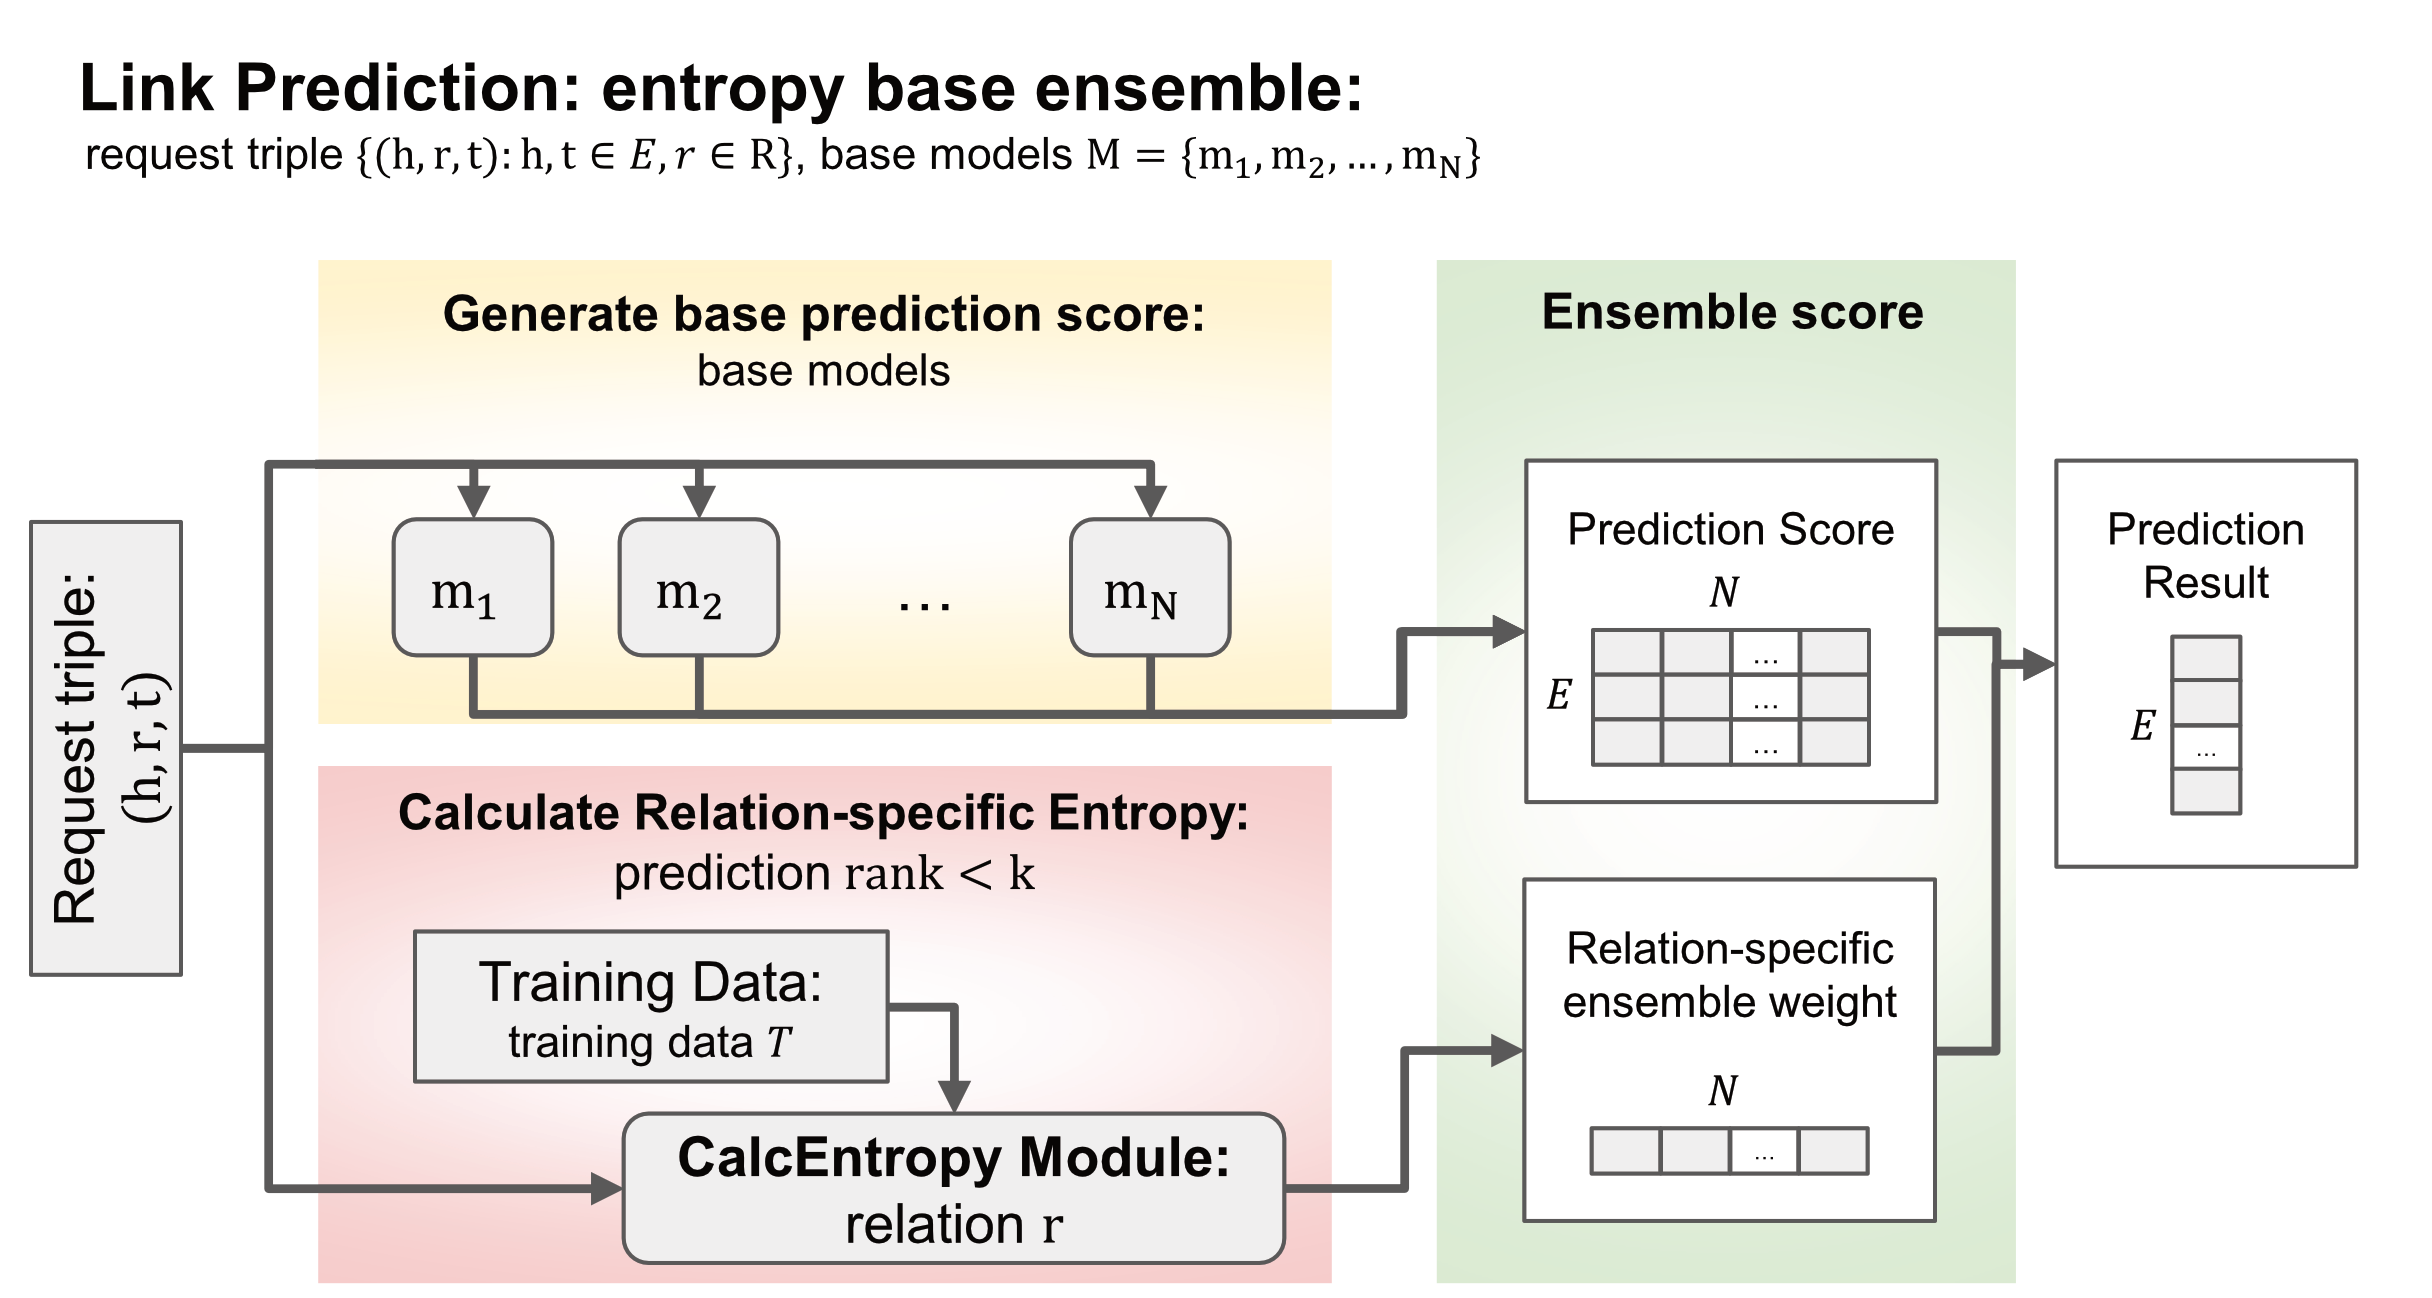
\includegraphics[width =0.75\textwidth]{Images/Figure1_v2.png}}{}
  \makeatother
  \caption{{Overview of link-prediction sequence: entropy base ensemble}}
  \label{fig:sysArch}
  \hfill
\end{figure*}
\egroup

In the this section, we detail the ERSE (knowledge graph Ensemble with Relation-Specific Entropy) approach, designed for enhancing link prediction in KGs. This approach is predicated on the hypothesis that the entropy of similarity distributions in feature vectors is a reliable indicator of a model's predictive performance. This method utilizes relation-specific entropy weights to ensemble multiple translation-based KGE. The process begins with the computation of base prediction scores for each model in the ensemble, followed by the calculation of relation-specific entropy. The entropy is derived from the distribution of feature vectors' similarity, which is based on the models' prediction ranking and training dataset. The calculated entropy then guides the determination of ensemble weights for each model. The final prediction score is a sum of the weighted scores from all models. This methodology is distinct in its focus on the entropy of feature vector similarity distributions within each model's vector space. The algorithmic phase, including inputs, outputs, and procedures, are elaborately illustrated in Figure ~\ref{fig:sysArch} and Algorithm ~\ref{alg:linkPredictOverview}. 

\begin{algorithm}[!htb]
    \caption{Link Prediction: entropy base ensemble}
    \label{alg:linkPredictOverview}
    \textbf{Input}: Request triple $\{(h, r, t) \;:\; h,t \in E, r \in R\}$, base models $\{\mathcal{M}_i \;:\; i \in N\}$, minimum number of vectors $minLen$ for weight reliability, type of entropy normalization $norm$, type of entropy $\mathit{type}$, type of distance $\mathit{dist}$, hit rank threshold $k$, and min-max range of normalization for prediction score $\delta^{s}$ and ensemble weight $\delta^{w}$.\\
    \textbf{Output}: Ensemble prediction Score $\mathcal{S}$.
    
    \begin{algorithmic}[1] %[1] enables line numbers    

        \Statex \hrulefill
        \Statex \textbf{Link-prediction sequence}
        \Statex \noindent$\overline{\makebox[\linewidth]{\text{Generates Base Prediction Score:} $s\acute{}$ \hfill}}$
        
        \State $s\acute{}_i \leftarrow \{\mathcal{N}_{\text{minmax}}(f^i(h, r, t), \delta^{S}) \;|\; \forall i \in N\}$    
        \Statex Calculate Relation-specific Entropy $\mathcal{H}$ and their number of resource vector: $resSize$.
        \State $\mathcal{H}, resSize \leftarrow \Call{CalcEntropy}{\mathcal{M}, r}$

        \Statex Ensemble for Final Prediction Score: $\mathcal{S}$.
        \State $\mathcal{W}^i \leftarrow \{\mathcal{N}_{norm}(\mathcal{H}^i, \delta^{W}) \;|\; resSize^{i}>minLen\}$

        \If{$\Call{Len}{\mathcal{W}} < 1$}
            \State $\mathcal{W}^i \leftarrow \{1\;|\; \forall i \in N\}$
        \EndIf
        
        \State $\mathcal{S} \leftarrow \sum_{m=1}^{N} s\acute{}_i \mathcal{W}i$
        \State \Return $\mathcal{S}$
        
        \Statex \hrulefill
        \Statex \noindent\underline{\hbox to \linewidth{\textbf{Relation-specific entropy calculation}\hfill}}

        \Function{CalcEntropy}{$\mathcal{M}, \hat{r}, k, type, dist, norm, \delta^w$}

            \State $\hat{T} \leftarrow \{(h,\hat{r},t)\;|\; \forall (h,\hat{r},t) \in T_{train}\}$
            \State $res^{i} \leftarrow \{\mathcal{V}^i(h,\hat{r},t) \;|\;\mathrm{avg}(\mathrm{rank}(h,\hat{r},t)) <k,$
            \Statex \hspace{3.5em}$(h,\hat{r},t) \in \hat{T}, \forall i \in N\}$
        
            \For{$i$ in $N$}
                \State ${res^{i}} \leftarrow \mathrm{drop}(res^{i}, \mathrm{min}(\mathrm{len}(res)))$
                \State $prob^{i} \leftarrow Probs(D_{\mathit{dist}}(res^{i}, res^{i}))$
                \State $\mathcal{E}^{i} \leftarrow \mathcal{H}^{\mathit{type}}(prob_r^m)$
                \State $resSize^{i} \leftarrow \mathrm{len}(res^{i})$  
            \EndFor
            \State \Return $\mathcal{E}, resSize$
        \EndFunction
    \end{algorithmic}
\end{algorithm}

\subsubsection{Request for Link-Prediction}

The ERSE takes as input a request triple $\{(h, r, t) : h, t \in E, r \in R\}$, where $E$ represents the set of entities including head and tail entities $h$ and $t$, and $R$ denotes the set of relations containing $r$. The algorithm also utilizes base models $\{\mathcal{M}_i : i \in N\}$, where $i$ is the index of base model and $N$ is the number of base models, along with a series of hyperparameters: 
\begin{itemize}
    \item $minLen$: Minimum number of feature vectors, critical for essential the reliability of the relationship-specific entropy as a performance indicator;
    \item $k$: Maximum prediction rank of feature vectors, critical for ensuring the reliability of the relationship-specific entropy as a performance indicator;
    \item $type$: Indicator of type of entropy formula to apply for relation-specific entropy computation;
    \item $norm$: Indicator of type of normalization method to apply for relation-specific entropy;
    \item $\delta^s$: The range for normalizing prediction scores;
    \item $\delta^w$: The range for normalizing ensemble weights.
\end{itemize}


\subsubsection{Generates Base Prediction Score}
In the initial phase of link prediction, each base model, denoted as $\mathcal{M}_i$, computes a prediction score $s\acute{}_i$ for the input triple using its respective score function $f(h,r,t)$. These scores undergo normalization by the min-max normalization $\mathcal{N}_{\text{minmax}}(X, \delta^s)$, define as: 
\begin{align}
\label{eq:NormMM}
    \mathcal{N}_{\text{minmax}}(X, \delta) = \delta_{min} + \delta_{scale}*\frac{x_{ij} - \min(X)}{\max(X) - \min(X)},
\end{align}%
where $X$ represents the set of data, with $\delta_{min}$ and $\delta_{scale}$ being the minimum value and scale value. The normalization process ensures that the scores from different models are scaled uniformly, facilitating a fair combination in the subsequent phases.
\\
\subsubsection{Calculate Relation-Specific Entropy}
To determine the ensemble weight specific to a relation, we calculate its relation-specific entropy, a core component of the algorithm, denoted as $\Call{CalcEntropy}$ in Algorithm \ref{alg:linkPredictOverview}. This function takes as input a set of base models $\mathcal{M}$, a target relation $\hat{r}$, and various hyperparameters: $k, type, dist, norm, \delta^w$. The function progresses through four pivotal stages: \textbf{Filtering Training Triple}, isolating relevant training triples for relation-specific analysis; \textbf{Relation-specific Feature Vectors}, identifying well-trained feature vectors from filtered data; \textbf{Pairwise Distances}, measuring pairwise distances to assess similarity; \textbf{Distribution Similarity of Feature Vector}, computing similarity distribution by the Burr distribution and probability density function; and \textbf{Relation-specific Entropy Calculation}, calculating relation-specific entropy to define the model's ensemble weights.
\\
\textbf{Filtering Training Triple}: To compute relation-specific entropy, we initiate by filtering triples from the training dataset $T_{train}$ that contain the target relation, denoted as $\hat{r}$, resulting in a filtered set $\hat{T}$. This step narrows the focus from a comprehensive to a specific relation, enabling us to infer the predictive performance of each model using $\hat{T}$ as a foundational resource. 
\\
\textbf{Relation-specific Feature Vectors}: Subsequently, Building on the filtered set $\hat{T}$, our algorithm further refines to identify subsets of well-trained prediction vectors (feature vectors) for each base model. For this, we apply a ranking threshold parameter $k$ to the link-prediction outcomes of each model on $\hat{T}$'s triples, selecting well-trained subset triples. Specifically, we calculate the link prediction rank $rank(h, \hat{r}, t)$ for each triplet in $\hat{T}$ involving the local target relation $\hat{r}$ by the $i$-th model. The feature vectors ${res^i ;:; i \in N}$, filtered by average rank and a predefined hit rank threshold $k$, are used to evaluate each model’s predictive accuracy for $\hat{r}$ in the sequence that follows. The extraction process varies among models. For example, in the TransE model~\cite{bordes2013translating}, it is defined as:
\begin{align}
\label{eq:PreV}
    \mathcal{V}^{TransE}(h, r, t) = \begin{cases}
            t-r & \text{, when head prediction} \\
            h+r & \text{, when tail prediction} \\
        \end{cases}.
\end{align}%
In this context, $res$ may contain multiple duplicates, especially in tail-predictions, as numerous triples $(h, \hat{r}, t)$ in $\hat{T}$ may only differ in $t$. Hence, these duplications are eliminated through the $\mathrm{avg()}$ function. Additionally, the varying lengths of each $res^i$ affect the subsequent entropy computation. Since ERSE computes its relation-specific entropy based on these $res^i$, discrepancies in length can negatively impact the performance and reliability of ensemble weights. Hence, as outlined in line 13 of Algorithm~\ref{alg:algorithm}, to ensure reliable ensemble weights indicative of each model's predictive performance for a relation, ERSE adjusts other $res^i$ to match the shortest length in the set, as executed by the $\mathrm{drop}$ function. 
\\
\textbf{Pairwise distances}: Our methodology extends to the examination of similarity distribution of feature vector through the measurement of pairwise distances. These distances, derived from feature vectors in the preceding step, are used to compute and utilize the probability density of these distances. We calculate pairwise distances $D_{\mathit{dist}}(res^{i}, res^{i})$ employing methods such as Euclidean and cosine distances, among other relevant metrics. In this study, we particularly explore the application of Euclidean and cosine distances. They are defined as follows:
\begin{align}
\label{eq:DistEu}
    \mathcal{D}_{\text{euclidean}}(A_i, A_j) = \sqrt{\sum_{k=1}^{m}(A_{ik} - A_{jk})^2},
\end{align}%
\begin{align}
\label{eq:DistLogit}
    \mathcal{D}_{\text{cosine}}(A_i, A_j) = 1 - \frac{\sum_{k=1}^{m}A_{ik} \times A_{jk}}{\sqrt{\sum_{k=1}^{m}A_{ik}^2} \times \sqrt{\sum_{k=1}^{m}A_{jk}^2}}.
\end{align}%
\\
\textbf{Distribution Similarity of Feature Vector}:
Our algorithm leverages the pairwise distances measured in the previous step to compute the similarity of feature vectors. This computed similarity distribution roles a critical role in determining the relation-specific entropy, which is the key return value of this function. For this purpose, we utilize a renowned probability density function (PDF), symbolized as $prob^i$, to analyze the similarity distribution of feature vectors specific to each model. The Burr distribution~\cite{burr1942cumulative} is given by:
\begin{align}
\label{eq:PDF}
    Probs(x; c, d) = cd \frac{x^{c-1}}{(1 + x^c)^{d+1}},        
\end{align}%
where $x$ is a non-negative variable, and $c > 0$ and $d > 0$ are the shape parameters of the distribution. The process of fitting the Burr distribution to our data involves estimating the parameters $c$ and $d$ that best describe the observed distribution of pairwise distances. This is typically achieved through a method of statistical inference, such as maximum likelihood estimation (MLE). MLE seeks to find the parameter values that maximize the likelihood function, which in turn indicates the most probable parameters given the observed data. Once the parameters of the distribution are estimated, the PDF is computed to evaluate the probability density of our data points. The PDF, as defined above, gives us a function that describes the likelihood of observing a given distance within our dataset. By applying the estimated parameters to this function, we can generate a probability distribution that accurately represents the pairwise distances in our feature vectors. As a example, Figure ~\ref{fig:pdfhist} illustrates an application of the Burr distribution in modeling the pairwise distances and the resultant probability density function. 
\bgroup
\begin{figure}[b!]
  \centering \makeatletter\IfFileExists{Images/Figure2.png}{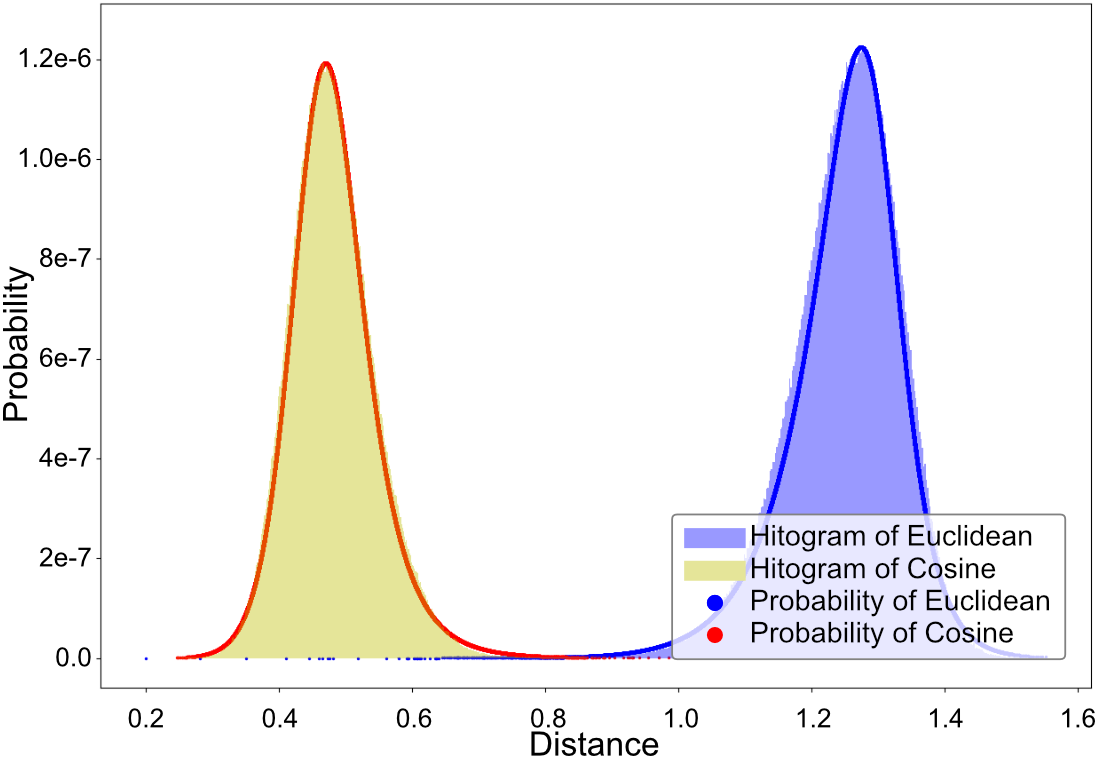
\includegraphics[width =0.48\textwidth]{Images/Figure2.png}}{}
  \makeatother
  \caption{{Compare of probability density function and pairwise distance histogram; TransD and relation $14$.}}
  \label{fig:pdfhist}
  \hfill
\end{figure}
\egroup
\\
\textbf{Relation-specific Entropy}: The final computation of relation-specific entropy is determined by measuring the entropy of similarity distribution. Specifically, the algorithm calculates the relation-specific entropy $\{\mathcal{H}^{i} \;:\; i \in N\}$, driven by the received parameter $type$. This implementation includes the adoption of various entropy types such as Shannon~\cite{shannon1948mathematical} and R\`enyi~\cite{renyi1961measures} entropy, difines as:
\begin{align}
    \label{eq:shannon}
    \mathcal{H}^{shannon}(X) = -\sum_{i} p(x_j) \log p(x_j), 
\end{align}%
\begin{align}
    \label{eq:renyi}    
    \mathcal{H}_{\alpha}^{r\acute{e}nyi}(X) = \frac{1}{1-\alpha} \log \left( \sum_{i} p(x_j)^\alpha \right).
\end{align}%
In these equation~\ref{eq:shannon} and ~\ref{eq:renyi}, $x_j$ represents the probability of occurrence of the $j$-th element in the distribution, and $\alpha$ is a parameter in the R\'enyi entropy that allows for the generalization of the Shannon entropy. The choice of entropy type influences how the diversity of the similarity distribution is quantified, thereby affecting the overall entropy calculation. The Shannon entropy is a measure of the average unpredictability in the distribution, whereas the R\'enyi entropy generalizes this concept, allowing for different levels of sensitivity to probabilities of occurrences in the distribution. The $\Call{CalcEntropy}$ function, which driven by parameter $type$ as a type of entropy, return the entropy result $\mathcal{H}$ and the resource size count $\{resSize^{i} \;:\; i \in N\}$. This provides a quantitative basis for determining the relation-specific ensemble weights in our model. The selection of the appropriate entropy type is based on the characteristics of the data and the specific requirements of the algorithm. The relation-specific entropy, thus calculated, plays a crucial role in the overall entropy-based ensemble learning process, providing a nuanced understanding of the similarity distribution within the model's feature vectors. This entropy measurement forms a pivotal component in assessing the predictive accuracy and reliability of the model for the targeted relations.

In our approach, the $\Call{CalcEntropy}$ function is a distinct and crucial component of the entropy-based ensemble learning process. It operates independently from the actual link prediction process, providing considerable flexibility in integrating pre-trained models. This independence allows for versatile combinations of base models. The function's design enables either a one-time computation during the link prediction phase or a pre-computation for each relation. This approach is strategically advantageous as it optimizes computational resources and significantly streamlines the link prediction process. By calculating relation-specific entropy, $\Call{CalcEntropy}$ offers a refined understanding of similarity distribution within the feature vectors of the model, thereby enhancing the predictive accuracy and reliability for targeted relations.
\\
\subsubsection{Ensemble for Final Prediction Score}
The final phase of the algorithm involves the establishment of ensemble weights and the computation of the prediction score, drawing upon the relation-specific entropy and base scores. This process is integral to the ERSE approach.
\\
\textbf{Determine of Ensemble Weights} For each model within the ensemble, we calculate relation-specific ensemble weights, denoted as $\mathcal{W}^i$. These weights are derived by normalizing the calculated relation-specific entropy, $\mathcal{H}$. Normalization methods such as min-max and logit are applied, tailored according to the normalization parameters $norm$ and $\delta^{W}$. The min-max normalization is defined in Equation~\ref{eq:NormMM}, while the logit normalization method is given by:
\begin{align}
\label{eq:NormLogit}
    \mathcal{N}_{\text{logit}}(X, \delta) =  \delta_{min} + \delta_{scale}*\log\left(\frac{x}{1 - x}\right),
\end{align}%
where $X$ represents the set of data, with $\delta_{min}$ and $\delta_{scale}$ being the minimum value and scale value. This normalization process excludes models whose number of resource vectors, denoted by $resSize^{i}$, is less than the predefined minimum length $minLen$.
\\
\textbf{Exception Weight Assignment} In cases where the ensemble lacks a sufficient number of weights ($\Call{Len}{\mathcal{W}} < 1$), a default weight of 1 is uniformly assigned across all models in the ensemble ($\mathcal{W}^i \leftarrow \{1\;|\; \forall i \in N\}$). This ensures that, in scenarios where relation-specific entropy is not substantial, each model in the ensemble contributes equally to the final prediction score.
\\
\textbf{Computation of Ensemble Prediction Score}: The ensemble prediction score, denoted as $\mathcal{S}$, is calculated by summing the products of each model's base prediction score, $s\acute{}_i$, with its corresponding weight, $\mathcal{W}^i$. 

The final outcome of this phase is the score $\mathcal{S}$, representing the aggregated predictive capability of the ensemble. This score reflects the combined insights from all models, adjusted for their respective relation-specific entropies and normalized weights. By integrating these elements, the algorithm aims to produce a more robust and accurate prediction outcome than any single model could achieve independently.

\section{Experiments and Results Analysis}
\label{Exper}
\subsection{Datasets}

In evaluate the performance of our approach, we utilized two benchmark KGs derived from Freebase~\cite{10.1145/1376616.1376746}: FB15K~\cite{NIPS2013_1cecc7a7} and FB15K237~\cite{toutanova-chen-2015-observed}. FB15K consists of a subset of knowledge triples from the extensive Freebase database, covering a range of topics including sports, actors, movies, and more. Most test triples in FB15K can be inferred by their inverse triples in the training dataset. In contrast, FB15K237, a modified version of FB15K, excludes inverse relations, presenting a more challenging scenario for link prediction as it demands more advanced modeling. Table ~\ref{tab:datasets} provides a comprehensive overview of these datasets.

\begin{table}[hbtp!]
{
    % \small
    \centering
    \begin{tabular}{cccccc}
        \toprule
        \textbf{Dataset} & \textbf{\#Ent} & \textbf{\#Rel} & \textbf{\#Train}  & \textbf{\#Valid.} & \textbf{\#Test}\\
        \midrule

        FB15K & 14951 & 1345 & 483142 & 50000 & 59071\\
        FB15K237 & 14541 & 237 & 272115 & 17535 & 20466\\
        
        \bottomrule
    \end{tabular}
    \caption{Score functions of translation-based embedding models}
    \label{tab:datasets}
}
\end{table}

\subsection{Experiment Settings}

\subsubsection{Implementation details}
The ERSE approach is implemented using Pytorch 2.0.0, on an Ubuntu 20.04 operating system, with a single NVIDIA RTX4090 GPU and an AMD Ryzen 9 5950x processor, backed by 64GB of RAM.

The study report the results of eight ERSE variants, distinguished by their combination of methods: entropy normalization (min-max or logit~\cite{berkson1944application}), entropy calculation (Shannon~\cite{shannon1948mathematical} or R\`enyi~\cite{renyi1961measures}), and pairwise distance measurement (Euclidean or cosine).

 We implemented and utilized an ensemble method, combining four typical translation-based KGE models, i.e. TransE, TransH, TansR and TransD, using the OpenKE~\cite{han-etal-2018-openke} framework for base model training before ensemble integration. The base models shared the same embedding dimension, with other hyperparameters set to OpenKE defaults. The implementation code and hyperparameters are available at ~\hyperlink{https://github.com/HW-Jeon/ERSE}{https://github.com/HW-Jeon/ERSE}, along with used hyperparameters.

\subsubsection{Baseline}
Follwing~\cite{WANG20221041}, ERSE's efficacy is also compared against two baselines to demonstrate our ensemble method's performance. The baselines include: (1) KGE methods: TransE~\cite{bordes2013translating}, TransH~\cite{wang2014knowledge}, TransR~\cite{lin2015learning}, TransD~\cite{ji2015knowledge};  (2) A general ensemble method, denoted as $\mathbf{ScoreSum}$, which aggregates the scores of each model, $\mathcal{S} \leftarrow \sum_{m=1}^{N} s\acute{}_i$.


% \subsection{Link Prediction}
% [† ]: results are taken from corresponding original paper

\subsection{Experimental Results of Link Prediction}
Following methodologies of various KGEs and the KGE ensemble approach ~\cite{WANG20221041}, We also employed link prediction to assess our ERSE model. Link prediction in KGs involves predicting missing head or tail entities $(h or t)$ in triplets $(h, r, t)$. To achieve this, In adherence to the widely-recognized filtered setting approach~\cite{bordes2013translating}, corrupted triplets in train, valid, and test sets were excluded, in sequence. We then scored these modified triplets and ranked them in descending order based on their scores. The evaluation focused not merely on identifying the top entity but on the rank of the correct entity. We used four metrics for this task: Hits@K (K=1, 3, 10) for accuracy in top K predictions, and Mean Reciprocal Ranking (MRR), with higher Hits@K and MRR indicating better performance.

Our experimental investigation yielded notable findings, as detailed in Tables ~\ref{tb:ExpResult} and ~\ref{tb:REResult}. These tables collectively present the outcomes of link prediction performance evaluations using the ERSE model, compared with various baseline models, across two datasets: FB15K and FB15K237.

\begin{center}
\begin{table*}[tp!]
{
    \centering 
    \begin{tabular}{c|c|cccc|cccc}
        \toprule
        \multicolumn{1}{c|}{} & \multicolumn{1}{c|}{\textbf{Dataset}} & \multicolumn{4}{c|}{\textbf{FB15K}} & \multicolumn{4}{c}{\textbf{FB15K237}} \\ 
        \midrule
        & \textbf{Model} & {MRR} & {Hits@1} & {Hits@3} & {Hits@10} & {MRR} & {Hit@1} & {Hit@3} & {Hit@10}\\
        \midrule
        & TransE & 0.3907 & 0.2700 & 0.4539 & 0.6126 & 0.2882 & 0.1905 & 0.3277 & 0.4859 \\ %& 0.2050 & 0.0129 & 0.3681 & 0.4773 \\
        & TransH & 0.4591 & 0.3287 & 0.5400 & 0.6890 & 0.289 & 0.1874 & 0.3316 & 0.4877  \\ %& 0.2028 & 0.0116 & 0.3701 & 0.4734 \\
        & TransR & 0.4649 & 0.3326 & 0.5487 & 0.6969 & 0.2911 & 0.1954 & 0.3292 & 0.4829 \\ %& 0.2138 & 0.0166 & 0.3894 & 0.4679 \\
        & TransD & 0.5139 & 0.3767 & 0.6098 & 0.7391 & 0.2915 & 0.1922 & 0.3311 & 0.4891 \\ %& 0.2040 & 0.0247 & 0.3551 & 0.4738 \\
        \midrule
        & \footnotesize	$\mathbf{ScoreSum}$ & 0.5158 & 0.3882 & 0.6005 & 0.7307 & 0.3177 & 0.2136 & 0.3629 & 0.5218 \\ %& 0.2154 & 0.0158 & 0.3909 & 0.4860 \\
        \midrule
        \multirow{4}{*}{\rotatebox[origin=c]{90}{ERSE}}
        % \hspace{0.01em}
        \multirow{4}{*}{\rotatebox[origin=c]{90}{\scriptsize($Shannon$)}}
        & \footnotesize $Euclidean+MinMax$ & 0.5337 & \underline{0.4056} & 0.6217 & 0.7467 & \textbf{0.3203} &  \textbf{0.2158} &  0.3658 &  0.5254 \\ %&&&& \\        
        & \footnotesize $Euclidean+Logit\ddagger$ & 0.5336 & 0.4053 & 0.6217 & 0.7463 & \underline{0.3203} &  \underline{0.2157} &  \textbf{0.3661} &  0.5250\\ %&&&& \\
        & \footnotesize $Cosine+MinMax$ & 0.5336 & 0.4054 & 0.6217 & \textbf{0.7467} & 0.3194 &  0.2145 & 0.365 &  0.5250\\
        & \footnotesize $Cosine+Logit$ & 0.5335 & 0.4051 & 0.6217 & 0.7463 & 0.3195 &  0.2145 &  0.3654 &  0.5254\\
        
        \midrule
        % \cmidrule(rl){1-1}
        
        \multirow{4}{*}{\rotatebox[origin=c]{90}{ERSE}}
        \multirow{4}{*}{\rotatebox[origin=c]{90}{\scriptsize($Re\acute{}nyi$)}}
        & \footnotesize $Euclidean+MinMax\dagger$ & \textbf{0.5337} & \textbf{0.4056} & 0.6217 & 0.7467 & 0.3203 &  0.2157 &  0.3655 &  0.5255 \\
        & \footnotesize $Euclidean+Logit$  & \underline{0.5337} & 0.4054 & 0.6217 & 0.7462 & 0.3202 & 0.2155 & \underline{0.3659} & 0.5254\\
        & \footnotesize $Cosine+MinMax$ & 0.5337 & 0.4055 & \underline{0.6217} & \underline{0.7467} & 0.3196 &  0.2146 &  0.3654 &  \underline{0.5255} \\ 
        & \footnotesize $Cosine+Logit$ & 0.5336 & 0.4052 & \textbf{0.6218} & 0.7463 & 0.3195 & 0.2143 & 0.3654 & \textbf{0.5258}\\

        
        \midrule
        & Relative $\uparrow$ & \textbf{3.47}\% & \textbf{4.49}\% & \textbf{3.53}\% & \textbf{2.19}\% & \textbf{0.81}\% & \textbf{1.01}\% & \textbf{0.78\%} & \textbf{0.67}\% \\
        
        \bottomrule
    \end{tabular}
    \caption{Results of link prediction on datasets FB15K and FB15K237. The \textbf{best} and \underline{second-best} scores in each column are emphasized. [$\dagger$]: best variant of ERSE for FB15K. [$\ddagger$]: best variant of ERSE for FB15K237. The row of Relative $\uparrow$ indicates the comparative link prediction performance between $\mathbf{ScoreSum}$ and the optimal variant of ERSE for each dataset. }
    \label{tb:ExpResult}
}
\end{table*}
\end{center}

\begin{center}
\begin{table*}[htb!]
{
    \centering
    \begin{tabular}{c|c|cccc|cccc}
        \toprule
        \multicolumn{1}{c}{} & \multicolumn{1}{c|}{\textbf{Dataset}} & \multicolumn{4}{c|}{\textbf{FB15K(Hits@10)}} & \multicolumn{4}{c}{\textbf{FB15K237(Hits@10)}} \\ 
        \midrule
        & \textbf{Model} & \textbf{1-to-1} & \textbf{1-to-N} & \textbf{N-to-1} & \textbf{N-to-N} & \textbf{1-to-1} & \textbf{1-to-N} & \textbf{N-to-1} & \textbf{N-to-N} \\
        \midrule
        & TransE & 0.8191 & 0.6389 & 0.6118 & 0.6057 & 0.5599 & 0.3623 & 0.4951 & 0.4858 \\ %& 0.2050 & 0.0129 & 0.3681 & 0.4773 \\
        & TransH & 0.8564 & 0.6813 & 0.6424 & 0.6959 & 0.5599 & 0.3461 & 0.4900 & 0.4985  \\ %& 0.2028 & 0.0116 & 0.3701 & 0.4734 \\
        & TransR & 0.9177 & 0.7173 & 0.6845 & 0.7476 & 0.5990 & 0.3256 & 0.4959 & 0.4915 \\ %& 0.2138 & 0.0166 & 0.3894 & 0.4679 \\
        & TransD & 0.8684 & 0.6919 & 0.6546 & 0.7011 & 0.5521 & 0.3531 & 0.4910 & 0.4997 \\ %& 0.2040 & 0.0247 & 0.3551 & 0.4738 \\
        \midrule
        & \footnotesize	$\mathbf{ScoreSum}$ & 0.9032 & 0.7185 & 0.6760 & 0.7396 & 0.5833 & 0.3797 & 0.5207 & 0.5338 \\ %& 0.2154 & 0.0158 & 0.3909 & 0.4860 \\
        \midrule
        \multirow{4}{*}{\rotatebox[origin=c]{90}{ERSE}}
        % \hspace{0.01em}
        \multirow{4}{*}{\rotatebox[origin=c]{90}{\scriptsize($Shannon$)}}
        & \footnotesize $Euclidean+MinMax$ & \textbf{0.9249} & 0.7279 & 0.6848 & 0.7577 & \textbf{0.5885} & 0.3778 & 0.5215 & 0.5385 \\ 
        & \footnotesize $Euclidean+Logit\ddagger$ & 0.9237 & 0.7278 & 0.6848 & 0.7571 & \textbf{0.5885} & 0.3801 & 0.5211 & 0.5379 \\ 
        & \footnotesize $Cosine+MinMax$ & \underline{0.9243} & \underline{0.7279} & 0.6843 & \textbf{0.7578} & \underline{0.5859} & 0.3809 & 0.5210 & 0.5379 \\ 
        & \footnotesize $Cosine+Logit$ & 0.9237 & 0.7278 & \underline{0.6849} & 0.7571 & \underline{0.5859} & \textbf{0.3821} & 0.5209 & 0.5385 \\ 
        
        \midrule
        % \cmidrule(rl){1-1}
        
        \multirow{4}{*}{\rotatebox[origin=c]{90}{ERSE}}
        \multirow{4}{*}{\rotatebox[origin=c]{90}{\scriptsize($Re\acute{}nyi$)}}
        & \footnotesize $Euclidean+MinMax\dagger$ & \underline{0.9243} & 0.7278 & 0.6847 & 0.7577 & \underline{0.5859} & 0.3778 & 0.5211 & \textbf{0.5388} \\ 
        & \footnotesize $Euclidean+Logit$  & 0.9237 & 0.7278 & 0.6848 & 0.7571 & \textbf{0.5885} & 0.3766 & \underline{0.5219} & 0.5385 \\ 
        & \footnotesize $Cosine+MinMax$ & \underline{0.9243} & \textbf{0.7281} & 0.6845 & \underline{0.7577} & \underline{0.5859} & \underline{0.3817} & 0.5211 & 0.5385 \\ 
        & \footnotesize $Cosine+Logit$ & 0.9237 & 0.7278 & \textbf{0.6850} & 0.7572 & \underline{0.5859} & 0.3790 & \textbf{0.5227} & \underline{0.5387} \\ 
        
        \bottomrule
    \end{tabular}
    \caption{Evaluation results on FB15K and FB15K237 by mapping properties of relations. The \textbf{best} and \underline{second-best} scores in each column are emphasized. [$\dagger$]: best variant of ERSE for FB15K. [$\ddagger$]: best variant of ERSE for FB15K237.}
    \label{tb:REResult}
}
\end{table*}
\end{center}

\subsubsection{Overall Performance on FB15K and FB15K237}
According to Table ~\ref{tb:ExpResult}, ERSE demonstrates notable superiority over baseline models, including TransE, TransH, TransR, and TransD, across multiple evaluation metrics. For both FB15K and FB15K237 datasets, ERSE variants exhibit substantial improvements in Mean Reciprocal Ranking (MRR) and Hits@K metrics (K=1, 3, 10). Specifically, the highest improvements variants (marked with $\dagger$ and $\ddagger$) observed in MRR are 3.47\% for FB15K and 0.81\% for FB15K237. Similar trends of enhancement are evident in Hits@1, Hits@3, and Hits@10, with the top variants outperforming the $\mathbb{ScoreSum}$ method: 4.49\% and 0.98\% in Hits@1, 3.53\% and 0.78\% in Hits@3, 2.19\% and 0.67\% in Hits@10, respectively.

\subsubsection{Performance of Properties of Relations}
Table ~\ref{tb:REResult} provides a deeper insight into ERSE's performance across different types of relations, categorized as 1-to-1, 1-to-N, N-to-1, and N-to-N, focusing on the Hits@10.  For both FB15K and FB15K237 datasets, ERSE's top variants (marked with $\dagger$ and $\ddagger$) consistently outperform the baseline models for all types of relations. Notably, the significant improvements are observed in 1-to-1 and N-to-N relations: 2.35\% and 0.89\% in 1-to-1 relations, 0.89\% and 0.77\% in N-to-N relations. However, a nuanced observation reveals that the performance increment in N-to-1 relationships on the FB15K237 dataset was marginal. Interestingly, for 1-to-1 relationships in the same dataset, the first variant did not surpass the $\mathbb{ScoreSum}$ model's performance, despite observing top performance increases among variants in MRR and Hits@1.

\subsubsection{Result Analysis}

The experimental outcomes, as detailed in Tables \ref{tb:ExpResult} and \ref{tb:REResult}, provide a comprehensive assessment of our ERSE model's performance in link prediction tasks. The ERSE model, when compared against standard baseline models (TransE, TransH, TransR, and TransD), exhibits a significant improvement in all evaluated metrics on both FB15K and FB15K237 datasets. Particularly, ERSE demonstrates the highest enhancements in Mean Reciprocal Ranking (MRR) and Hits@K metrics (K=1, 3, 10) across these datasets. The most significant improvements in MRR are 3.47\% for FB15K and 0.81\% for FB15K237. Furthermore, ERSE variants outperform the $\mathbb{ScoreSum}$ method in Hits@1, Hits@3, and Hits@10 with notable margins.

Delving into relation-specific performance (Table \ref{tb:REResult}), ERSE shows consistent superiority over baseline models in diverse relation types: 1-to-1, 1-to-N, N-to-1, and N-to-N. The most substantial performance gains are observed in 1-to-1 and N-to-N relations: 2.35\% and 0.89\% in 1-to-1 relations, and 0.89\% and 0.77\% in N-to-N relations, respectively, across both datasets. It is noteworthy that the improvement in N-to-1 relationships for FB15K237 is marginal, and for 1-to-1 relationships in the same dataset, the first variant of ERSE does not surpass the $\mathbb{ScoreSum}$ model. We suspect that this stems from the nature of the voting ensemble, where the selection of the base model matters~\cite{a13010026}. These results indicate the effectiveness of the ERSE model in enhancing link prediction accuracy, more various KGE models, such as RotatE, ComplEx, and the need for ensemble. 

The study, while affirming ERSE's effectiveness, acknowledges limitations. Presently, ERSE is limited to translational-distance-based KGEs and lacks hyperparameter tuning in its foundational model. To resolve these limitations and further investigate the unexpected results in previous relational property experiments, future research is necessary with involve hyperparameter-tuned KGEs from different categories as the base model.

\section{Conclusion}
\label{Conclusion}
The paper presents a novel approach focusing on relation-specific entropy as an ensemble weight for KGE. The core concept is that the entropy of feature vector similarity distributions reliably indicate the inference performance of KGEs. This approach utilizes ensemble weights determined by the entropy of distribution similarity, leveraging embedded feature vectors from each base model's representation space. This method has shown to enhance predictive accuracy substantially. Theoretical foundations of the study are confirmed through experiments on benchmark datasets FB15K and FB15K237, where the ERSE model consistently outperforms existing models and general ensemble methods across key metrics. However, limitations also observed which related to base models. In the future, we will solve and analysis these limitations, and apply to other machine learning model ensembles.

\section*{Acknowledgments}

%% The file named.bst is a bibliography style file for BibTeX 0.99c
\bibliographystyle{named}
\bibliography{ijcai23}

\end{document}
